\documentclass[conference]{IEEEtran}
\IEEEoverridecommandlockouts

\usepackage{algorithm}
\usepackage{algorithmic}
\usepackage{graphicx}
\usepackage{booktabs}
\graphicspath{{../assignment/pics/}}

% ==== Essential Mathematical and Scientific Packages ====
% Package for mathematical symbols, equations, and AMS-specific features
\usepackage{amsmath,amssymb,amsfonts}
% Package for writing algorithms in pseudo-code
\usepackage{algorithmic}
% Package for including and manipulating graphics/images
\usepackage{graphicx}
% Package for special text symbols like degree signs, currency symbols
\usepackage{textcomp}
% Package for colored text and background
\usepackage{xcolor}
% Package for creating subfigures with individual captions
\usepackage{subcaption}
% Package for professional-looking tables with booktabs rules
\usepackage{booktabs}
% Package for typesetting SI units and numbers consistently
\usepackage{siunitx}

% ==== Bibliography Setup (biblatex with Harvard style) ====
% Configure biblatex with specific settings:
% - style=authoryear: Harvard-like citation style
% - backend=biber: Use biber backend instead of traditional BibTeX
% - dashed=false: Don't use dashes for repeated authors
% - maxnames=999: Show all author names (no "et al." truncation)
% - maxcitenames=3: Show up to 3 authors in citations
% - giveninits=true: Use initials for given names
% - urldate=long: Full date format for URL access dates
% - uniquename=false: Don't disambiguate similar author names
% - uniquelist=false: Don't disambiguate similar author lists
\usepackage[style=authoryear, backend=biber, dashed=false, maxnames=999, maxcitenames=3, 
    giveninits=true, urldate=long, uniquename=false, uniquelist=false]{biblatex}

% Specify the bibliography database file
\addbibresource{references.bib}

% ==== Citation Format Customization ====
% Add a comma between author name and year in citations
\renewcommand*{\nameyeardelim}{\addcomma\space}

% ==== Bibliography Entry Format Customization ====
% Remove quotes from titles for various entry types
\DeclareFieldFormat[article,inbook,incollection,inproceedings,patent,thesis,unpublished]{title}{#1}
% Make journal titles italic
\DeclareFieldFormat{journaltitle}{\emph{#1}}

% Format online resources according to Harvard style
\DeclareFieldFormat[online]{title}{\emph{#1}}
\DeclareFieldFormat{url}{Available from: \url{#1}}
\DeclareFieldFormat{urldate}{[Accessed #1]}

% Custom driver for online entries
\DeclareBibliographyDriver{online}{%
  \usebibmacro{bibindex}%
  \usebibmacro{begentry}%
  \usebibmacro{author/editor}%
  \setunit{\labelnamepunct}\newblock
  \usebibmacro{date}%
  \setunit{\addspace}\newblock
  \usebibmacro{title}%
  \newunit\newblock
  \printfield{url}%
  \setunit{\addspace}\newblock
  \printurldate
  \usebibmacro{finentry}%
}

% ==== Journal Entry Format Customization ====
% Customize how journal entries are formatted:
% - Includes journal name
% - Handles series information
% - Formats volume, number, and issue information
\renewbibmacro*{journal+issuetitle}{%
  % Print the journal name
  \usebibmacro{journal}%
  % Handle optional series information
  \iffieldundef{series}
    {}
    {\newunit
     \printfield{series}}%
  % Add volume, number, and electronic ID
  \usebibmacro{volume+number+eid}%
  % Add comma and space before date
  \setunit{\addcomma\space}%
  % Add issue and date information
  \usebibmacro{issue+date}%
  % Add colon and space before issue number
  \setunit{\addcolon\space}%
  % Print the issue
  \usebibmacro{issue}%
  % Prepare for next unit
  \newunit}

% ==== Author Name Format Customization ====
% Define how author names should be formatted:
% - Family name first
% - Given name as initials
% - Handle prefixes (von, van, etc.) and suffixes (Jr., III, etc.)
\DeclareNameFormat{sortname}{%
  \nameparts{#1}%
  \usebibmacro{name:family-given}
    {\namepartfamily}
    {\namepartgiveni}
    {\namepartprefix}
    {\namepartsuffix}%
}
% Apply this format as the default for all names
\DeclareNameAlias{default}{sortname}

% ==== Name List Format Customization ====
% Define how multiple author names are separated
% Add comma and space between multiple names
\DeclareDelimFormat{multinamedelim}{\addcomma\space}
% Use the same delimiter for the final name in the list
\DeclareDelimAlias{finalnamedelim}{multinamedelim}

% ==== Bibliography Printing Command ====
% Define a custom command to print bibliography with optional parameters
% #1 allows passing additional options to \printbibliography
\newcommand{\printbibsection}[1][]{\printbibliography[title=References,#1]} 

\begin{document}

\title{Localisation and Mapping Assignment Report}

\author{
\IEEEauthorblockN{
    Filip Hanuš,
}
\IEEEauthorblockA{
    School of Engineering, College of Art, Technology and Environment,\\
    University of the West of England, Bristol, UK\\
    Email: filip2.hanus@live.uwe.ac.uk}
}

\maketitle

\section{Introduction}
This report presents the outcomes of the Localisation and Mapping assignment for the Advanced Vision for Localisation and Mapping module.

\section{Task 1: Robot Control} 
\begin{itemize}
  \item \textbf{Requirements:} Implement a closed-loop ROS/MATLAB controller to explore at least 50\% of the environment without collisions and provide a ground-truth path figure.
  \item \textbf{Reflection:} Achieved 100\% coverage without collisions but found tuning the forward and centring gains challenging, causing small oscillations at the center turns (around markers 3 and 7).
  \item \textbf{Achievements \& Challenges:} Successfully navigated the maze collision-free; required a 0.1 m hysteresis to stabilise the controller at sharp turns. Robot path is shown in Figure~\ref{fig:task1_route}.
\end{itemize}
\begin{figure}[ht]
  \centering
  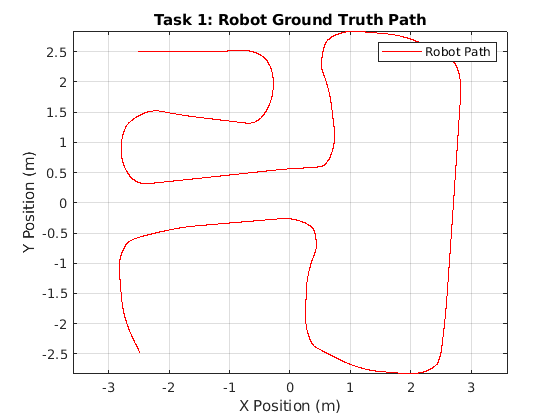
\includegraphics[width=\linewidth]{images/Task1_Route.png}
  \caption{Ground truth path of the robot exploring the environment.}
  \label{fig:task1_route}
\end{figure}

\section{Task 2: Motion Model}
\begin{itemize}
  \item \textbf{Requirements:} Generate a noisy pose estimate using a velocity motion model with the given noise parameters and include an overlay figure of ground truth vs noisy path.
  \item \textbf{Reflection:} The motion model effectively captured drift, and repeated runs showed consistent final deviations, highlighting the model's stability yet accumulating error.
  \item \textbf{Achievements \& Challenges:} Implemented \texttt{sample\_velocity\_motion\_model} correctly and saved outputs in \texttt{task2\_data.mat}. Robot path is shown in Figure~\ref{fig:task2_route}.
\end{itemize}
\begin{figure}[ht]
  \centering
  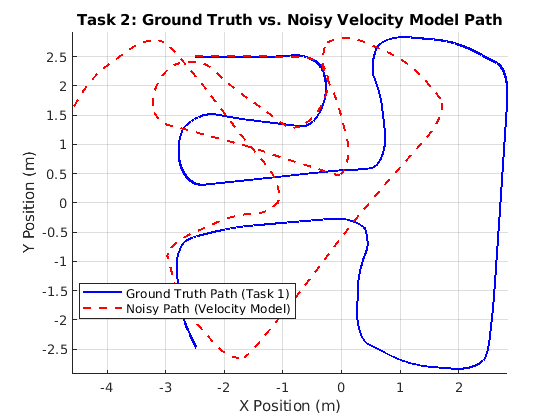
\includegraphics[width=\linewidth]{images/Task2_Route.png}
  \caption{Overlay of ground truth path (solid blue) and noisy pose estimate (dashed red) generated by the velocity motion model.}
  \label{fig:task2_route}
\end{figure}

\section{Task 3: Mapping} 
\begin{itemize}
  \item \textbf{Requirements:} Build an occupancy grid from ground-truth poses and LiDAR data, plus map ArUco marker positions; include two figures (occupancy grid and ArUco map).
  \item \textbf{Reflection:} The occupancy grid displays walls, produces a little bit of noise at turns; ArUco detections were robust overall but low-angle views of markers 4 and 5 yielded less than 70 observations.
  \item \textbf{Achievements \& Challenges:} Packaged all datasets in `task3\_dataset/`; adjusted detection thresholds to balance false negatives and spurious detections but accepted lower sample counts for occluded markers. Occupancy grid is shown in Figure~\ref{fig:task3_occupancy_grid_map}. ArUco marker map is shown in Figure~\ref{fig:task3_aruco_marker_map}.
\end{itemize}
\begin{figure}[ht]
  \centering
  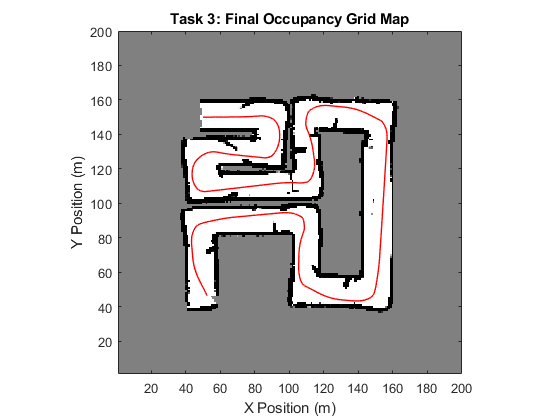
\includegraphics[width=\linewidth]{images/task3_occupancy_grid_map.png}
  \caption{Occupancy grid map generated from ground truth pose and LiDAR data.}
  \label{fig:task3_occupancy_grid_map}
\end{figure}

\begin{figure}[ht]
  \centering
  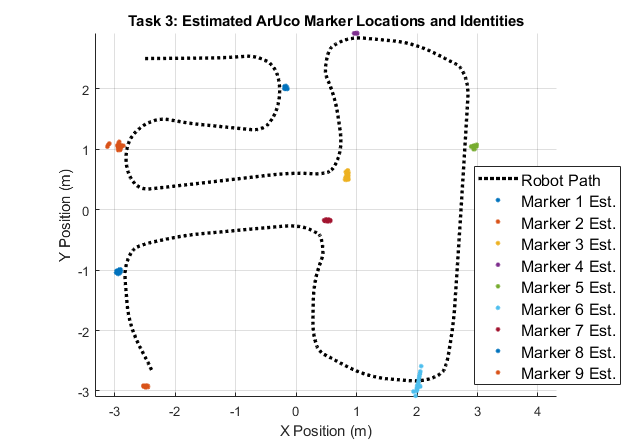
\includegraphics[width=\linewidth]{images/task3_aruco_marker_map.png}
  \caption{Estimated ArUco marker locations and identities overlaid on the robot path.}
  \label{fig:task3_aruco_marker_map}
\end{figure}

\section{Task 4: Extended Kalman Filter Localisation} 
\begin{itemize}
  \item \textbf{Requirements:} Fuse noisy odometry and known ArUco landmark measurements via an Extended Kalman Filter; provide path overlay and L2-norm error figures.
  \item \textbf{Reflection:} EKF successfully mitigated drift overall, but around markers 4-5 low detection counts induced over-correction in the estimate.
  \item \textbf{Achievements \& Challenges:} Derived and validated analytical Jacobians; encountered sensitivity to sparse landmark observations causing occasional jumps in the filter update. Robot path is shown in Figure~\ref{fig:task4_paths}. L2 norm error is shown in Figure~\ref{fig:task4_l2norm}.
\end{itemize}

\begin{figure}[ht]
  \centering
  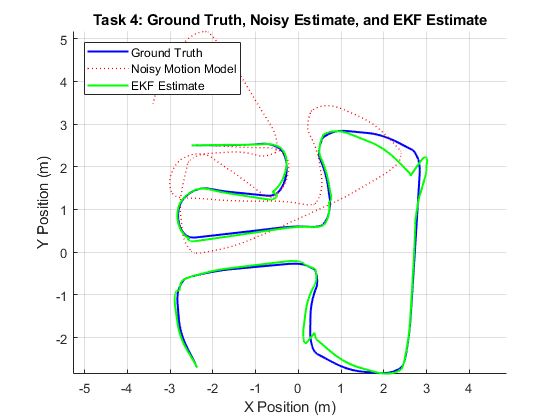
\includegraphics[width=\linewidth]{images/Task4_Paths.png}
  \caption{Ground truth (blue), noisy motion model (red dashed) and EKF estimate (green).}
  \label{fig:task4_paths}
\end{figure}

\begin{figure}[ht]
  \centering
  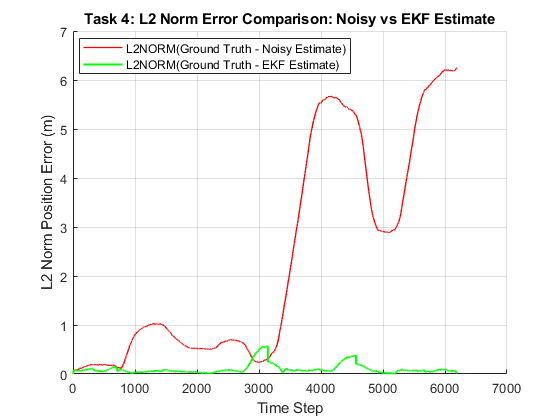
\includegraphics[width=\linewidth]{images/Task4_L2NORM.png}
  \caption{L2 norm error of noisy estimate (red) vs EKF estimate (green) over time.}
  \label{fig:task4_l2norm}
\end{figure}

\section{Task 5: Particle Filter Localisation} 
\begin{itemize}
  \item \textbf{Requirements:} Implement a Particle Filter, and include trajectory and L2-norm error figures.
  \item \textbf{Reflection:} PF matched EKF accuracy but at much longer runtime; reducing from 100\,000 to 1\,000 or 100 particles increased peak error rapidly.
  \item \textbf{Achievements \& Challenges:} Deployed systematic resampling effectively; balanced error vs computational load by benchmarking multiple particle counts. Particle filter path is shown in Figure~\ref{fig:task5_paths}. L2 norm error is shown in Figure~\ref{fig:task5_l2norm}.
\end{itemize}

\begin{figure}[ht]
  \centering
  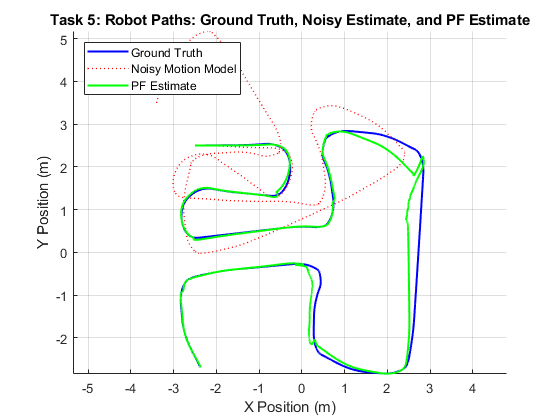
\includegraphics[width=\linewidth]{images/Task5_Paths_100kp.png}
  \caption{Particle filter localisation performance compared to ground truth and noisy estimate.}
  \label{fig:task5_paths}
\end{figure}

\begin{figure}[ht]
  \centering
  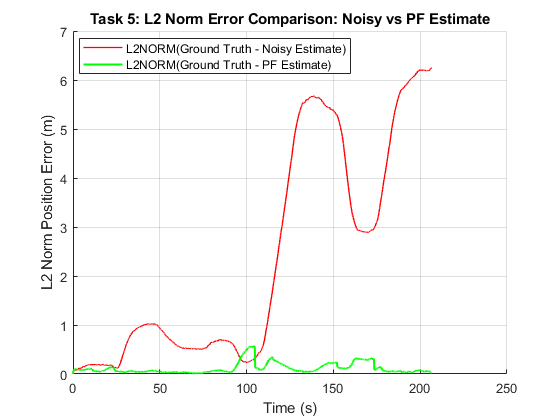
\includegraphics[width=\linewidth]{images/Task5_L2NORM_100kp.png}
  \caption{L2 norm error of noisy estimate (red) vs PF estimate (green) over time.}
  \label{fig:task5_l2norm}
\end{figure}

\section{Conclusion}
The exploration achieved over 100\% coverage without collisions, and the mapping pipeline generated occupancy grids and ArUco marker positions. The Extended Kalman Filter minimised the pose error compared to raw odometry, while the Particle Filter offered a very similar performance at the cost of higher computational expense.

%\printbibsection

\renewcommand{\thesection}{\Alph{section}}

% Appendix: code repository link
\section*{Appendix: Code Repository}
The MATLAB code and supporting files for this assignment are available at:
\url{https://github.com/FHanus/robot-localisation-and-mapping}


\end{document}